\documentclass[UTF8,a4paper,11pt]{ctexart}
\usepackage{titlesec}
%\titleformat{\section}{\flushleft\bfseries\Large}{\thesection}{1em}{}
\usepackage{CJKutf8}
\usepackage{graphicx}
\usepackage[unicode]{hyperref}
\usepackage{xcolor}
\usepackage{cite}
\usepackage{indentfirst}
\usepackage{blindtext}
\usepackage{ctex}
\parindent=2em
%%设置页边距
\usepackage[left=2.5cm,right=2.5cm,top=3cm,bottom=2.0cm]{geometry}
%%设置页眉页脚
\usepackage{fancyhdr}
\pagestyle{fancy}
\renewcommand\headrulewidth{2pt}       % 页眉横线
\lhead{}
\rhead{}
\fancyhead[C]{北京科技大学硕士学位研究生选题报告及文献综述}
\fancyfoot[C]{\thepage}%这条语句可以让页码出现在下方
\renewcommand{\headrulewidth}{0.4pt}
%%模板:	https://www.jianshu.com/p/3e842d67ada2
%%目录
\usepackage[section]{placeins}%避免浮动体跨过\section等章节标题
\usepackage[]{hyperref}%%目录引用等超链接
\hypersetup{colorlinks=true}
\usepackage[super]{gbt7714}%参考文献角标数字顺序编
\usepackage{setspace}

\usepackage{enumerate}
\usepackage{enumitem}
\setlist[enumerate,1]{label=(\arabic*),labelsep=1.5mm,topsep=0mm,itemsep=0mm}
\setitemize[1]{labelsep=1.5mm,itemsep=0mm,topsep=0mm}
\usepackage{amsfonts}
%%参考文献 设置
\bibliographystyle{ }
\usepackage{natbib}
\setlength{\bibsep}{0.5ex}

\begin{document}
\begin{sloppypar}
	\thispagestyle{empty}
	\begin{center}
		\hspace{1em}
		\vspace{1cm}
		\fontsize{24pt}{2em}\kaishu 北京科技大学\\
		\hspace{1em}
		\vspace{0.5cm}
		\fontsize{32pt}{15pt}\textbf{硕士学位研究生}\\ 
		\hspace{1em}
		\vspace{0.9cm}
		\fontsize{32pt}{15pt}\textbf{选题报告及文献综述}\\
		\hspace{1em}
		\vspace{0.5cm}
		\fontsize{24pt}{12pt}课题名称\\
		\fontsize{24pt}{12pt}深度学习在计算机视觉方面的应用研究研究\\
		\begin{figure}[htbp]
			\centering
			
\includegraphics[width=6cm]{./image/logo.png}
		\end{figure}
		\begin{table}[htbp]
			\songti
			\centering
			\makeatletter
			\newcommand\dlmu[2][4cm]{\hskip1pt\underline{\hb@xt@ #1{\hss#2\hss}}\hskip3pt}
			\makeatother
			\hspace{1em}
			\vspace{0.5cm}
			\begin{tabular}{cc}
				\vspace{0.5cm}
				\Large{指导教师:} & \dlmu[8cm]{\Large{大牛}}       \\
				\vspace{0.5cm}
				\Large{单\qquad 位:}   & \dlmu[8cm]{\Large{计算机与通信工程学院}} \\ 
				\vspace{0.5cm}
				\Large{学\qquad 号}:   & \dlmu[8cm]{\Large{210210000}}  \\ 
				\vspace{0.5cm}
				\Large{作\qquad 者:}   & \dlmu[8cm]{\Large{张三}}        \\
				\vspace{0.5cm}
				\Large{专业名称:} & \dlmu[8cm]{\Large{计算机科学与技术} }   \\ 
				\vspace{0.5cm}
				\Large{入学时间:} &  \dlmu[8cm]{\Large{2020年9月}}    \\
			\end{tabular}
		\end{table}
	\large{2021年1月}
	\end{center}
%目录
	\newpage
	\songti
	\thispagestyle{empty}
	\tableofcontents
	
	\newpage
	%正文
	\songti
	\CTEXsetup[format={\Large\bfseries}]{section}%标题左对齐
	\setcounter{page}{1}
	
	\section{课题研究背景和意义}
	
	\subsection{研究背景}
	
	深度学习在计算机视觉方面有着广泛的应用
	
	\subsection{研究目的及意义}
	
	图像分类检测的方面,深度学习的提出让这些视觉任务飞速发展
	
	
	
	\section{文献综述}
	\subsection{引言}
	图像分类是计算机视觉的基础任务之一,图像分类算法主要是。。。。。。为了实现好的分类效果,研究者不断改进和提出新的方案。。。。。
	
	\subsection{传统图像分类算法}
	在传统计算机视觉中,通过关键点边缘提取等算法。。。。
	
	\subsubsection{手工特征算法}
	
	
	\begin{figure}[htbp]
		\centering
		\begin{minipage}[t]{0.48\textwidth}
			\centering
			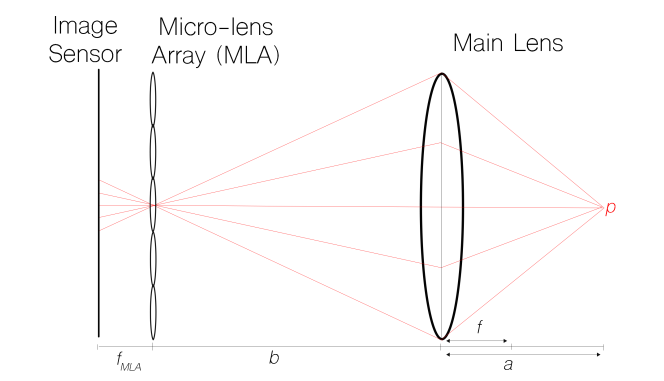
\includegraphics[width=6cm]{./image/plenoptic1.0.png}
			\caption{全光相机1.0模型}
			\label{fig:label}
		\end{minipage}
		\begin{minipage}[t]{0.48\textwidth}
			\centering
			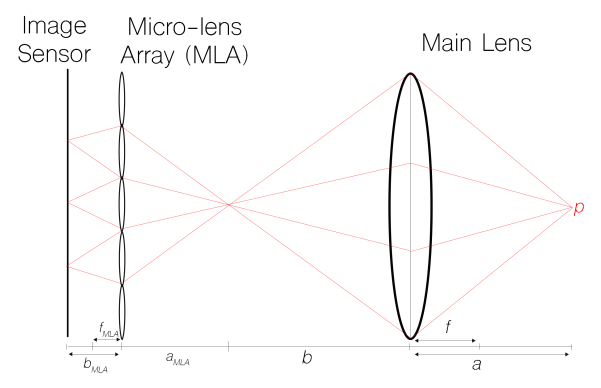
\includegraphics[width=6cm]{./image/plenoptic2.0.png}
			\caption{全光相机2.0模型}
			\label{fig:label}
		\end{minipage}
	\end{figure}
	
	
	
	\subsubsection{自适应特征提取算法}
	类似自适应分割算法等\cite{wang2020deep,thelightfield}。。。。
	
	\begin{table}[h]
		\centering
		\footnotesize
		\caption{图像分类数据集}
		\vspace{10pt}
		\begin{tabular}{ccc}
			\hline
			数据集                   & 空间分辨率          &角度分辨率            \\ \hline
			Stanford Multiview    & 541×376                 & 3$\sim$5视点       \\
			Stanford Lytro        & 625×434                 & 15×15            \\
			Stanf11111ord Archive(new) & 640×1024$\sim$1536×1152 & 17×17            \\ 
			Stanford Archive(old) & 128×128$\sim$256×256    & 8×8$\sim$32×32   \\
			LFSD                  & 379×379                 & 11×11            \\
			LCAV-31               & 301×301                 & 10×10            \\
			HCI old              & 628×768926×1024         & 9×9              \\
			HCI new              & 512×512                 & 9×9              \\
			EPFL                  & 625×434                 & 15×15            \\
			Synthetic             & 525×840/384×512         & 5×5/7×7          \\
			JPEG Pleno            & 170×1141$\sim$536×1152  & 15×15$\sim$20×20 \\
			Raytrix               & .......                & 32×32            \\ \hline
		\end{tabular}
		\label{bs5}
	\end{table}
	
	\subsection{基于学习的图像分类}
	\subsubsection{深度学习基本概念}
	
	
	\subsubsection{图像分类算法综述}
	图像分类。。。。。。
	\begin{equation}
		I_x = \mathcal{D}(I_y;\delta)
	\end{equation}
	

	\subsubsection{数据集}
	ImageNet
	
	
	\subsubsection{模型设计}
	
	虽然目前分类已经达到了一定的效果,但是。。。。
	
	\begin{figure}[htbp]
		\centering
		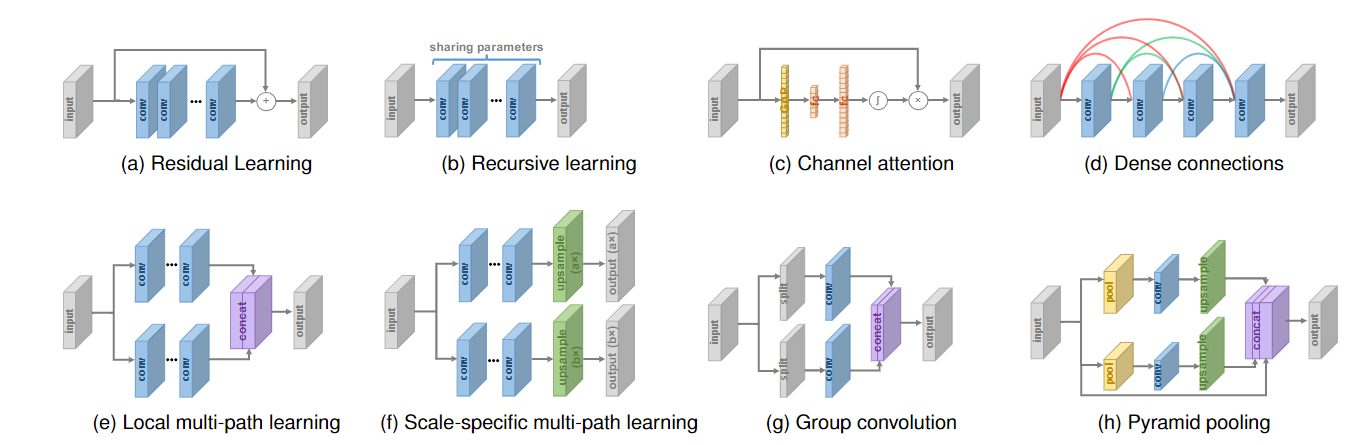
\includegraphics[width=13cm]{./image/network.png}
		\caption{图像分类}
		\label{fig:label}
	\end{figure}
	
	\subsubsection{训练策略}
	
	\begin{equation}
		\mathcal{L}_{l1}(\hat{I}, I)=\frac{1}{hwc}\Sigma_{i,j,k}|\hat{I}_{i,j,k}-I_{i,j,k}| 
	\end{equation}
	\begin{equation}
		\mathcal{L}_{l2}(\hat{I}, I)=\frac{1}{hwc}\Sigma_{i,j,k}(\hat{I}_{i,j,k}-I_{i,j,k})^2
	\end{equation}

	则内容损失表示为两个图像的第$l$层高级特征之间的欧式距离,如下内容损失的计算表达式为:
	\begin{equation}
		\mathcal{L}_{content}(I,\hat{I};\psi,l)=\frac{1}{h_l w_l c_l}\sqrt{\Sigma_{i,j,k}(\psi_{i,j,k}^{(l)}(\hat{I})-\psi_{i,j,k}^{(l)}(I))^2}
	\end{equation}

	而patch size的选用是一种经验性选择,因此使用纹理损失进行网络训练具有不稳定性。纹理损失表示为:
	\begin{equation}
		\mathcal{L}_{texture}(I,\hat{I};\psi,l)=\frac{1}{c_l^2}\sqrt{\Sigma_{i,j}(G_{ij}^{(l)}(I)-G_{ij}^{(l)}(\hat{I}))^2}
	\end{equation}
	
	除了以上损失函数外,还有基于生成对抗网络的损失函数、循环一致性损失、全局变化损失以及基于先验信息的损失等。
	
	\subsubsection{自监督学习算法}
	现有的超分辨率作品大多侧重于使用监督学习,即使用匹配的高低分辨率的图像对进行学习。但由于难以收集相同场景但分辨率不同的图像。
	
	\begin{figure}[htbp]
		\centering
		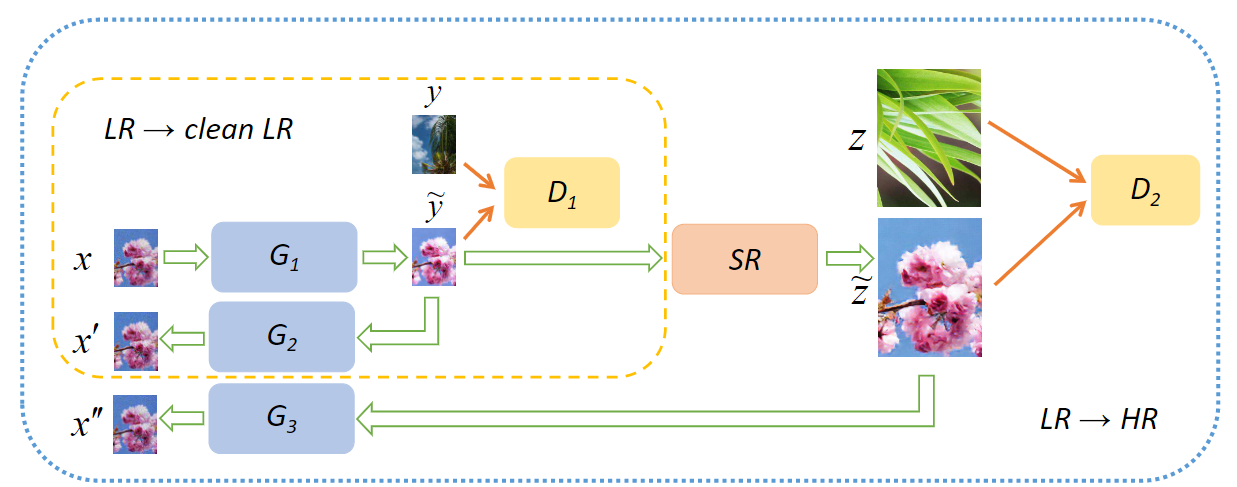
\includegraphics[width=13cm]{./image/GAN.png}
		\caption{基于GAN的超分辨率网络}
		\label{fig:label}
	\end{figure}
	
	
	\subsection{图像分类模型加速} %%重点
	GPU(Graphic Processing Unit)这个概念是由Nvi。。。。。
	随着GPU的不断更新,其计算能。。。。
	
	\begin{figure}[htbp]
		\centering
		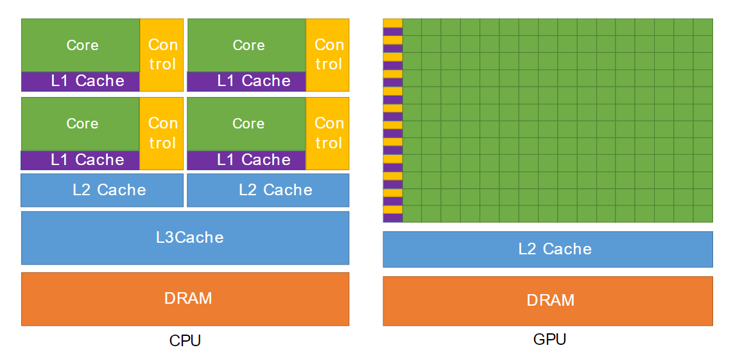
\includegraphics[width=14cm]{./image/gpu.png}
		\caption{GPU与CPU之间的区别}
		\label{fig:label}
	\end{figure}
	
	\subsubsection{CUDA架构}
	CUDA并行计算架构最主要的优点是可。。。。。
	
	在CUDA编程中,一个并行程序分为。。。。。。
	
	\begin{figure}[htbp]
		\centering
		\begin{minipage}[t]{0.48\textwidth}
			\centering
			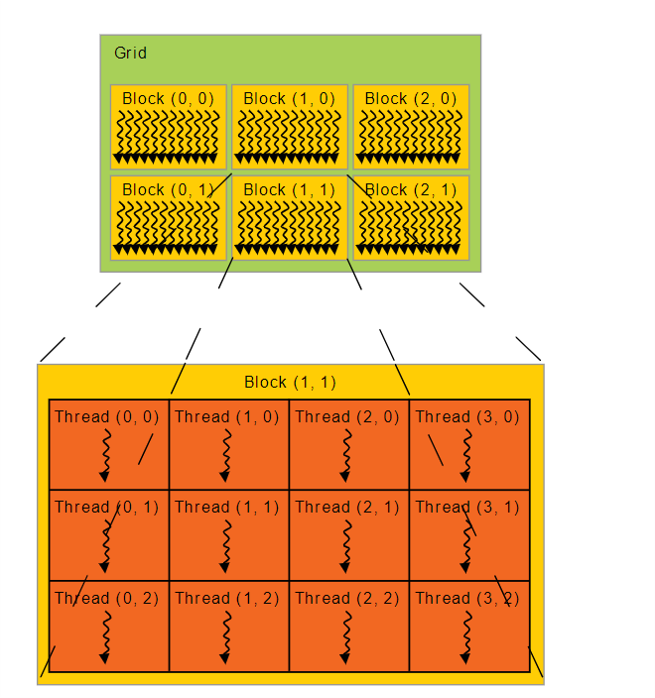
\includegraphics[width=8cm,height=10cm]{./image/thread.png}
			\caption{线程模型}
			\label{fig:label}
		\end{minipage}
		\begin{minipage}[t]{0.48\textwidth}
			\centering
			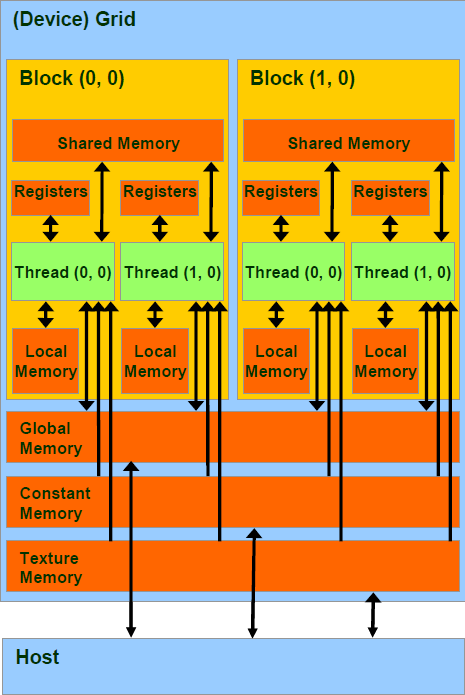
\includegraphics[width=8cm,height=10cm]{./image/memory.png}
			\caption{存储结构}
			\label{fig:label}
		\end{minipage}
	\end{figure}
	
	
	\subsubsection{CUDA深度学习加速计算上的应用}
	目前CUDA技术。。。。。
	
	\section{研究内容与方法}
	针对目前。。。。。
	
	
	\subsection{研究内容} 
	为了解决。。。问题, 拟采用。。。。
	
	
	\subsubsection{内容1}
	分类算法。。。
	
	\subsubsection{内容2}
	加速。。。
	
	\subsection{研究难点}
	\begin{enumerate}
		\item 特征提取
		\item 数据增强;
		\item 模型加速;
		\item 。。。。。。
	\end{enumerate}
	\subsection{研究方法与技术路线}
	为了解决。。。目前已有。。。不足在于。;。。。,可改进在于。。。。。
	
	
	\begin{enumerate}
		\item 本课题首先对相关文献进行调研。。。。。
		
		\item 复现现。。。。。;
		\item 研究。。。。。
		\item 研究。。。。。
		%\item 针对光场图像的角度分辨率进行超分辨率研究,实现从稀疏光场图像中恢复出稠密光场图像;
		\item 。。。。算法加速。
	\end{enumerate}
	\begin{figure}[htbp]
		\centering
		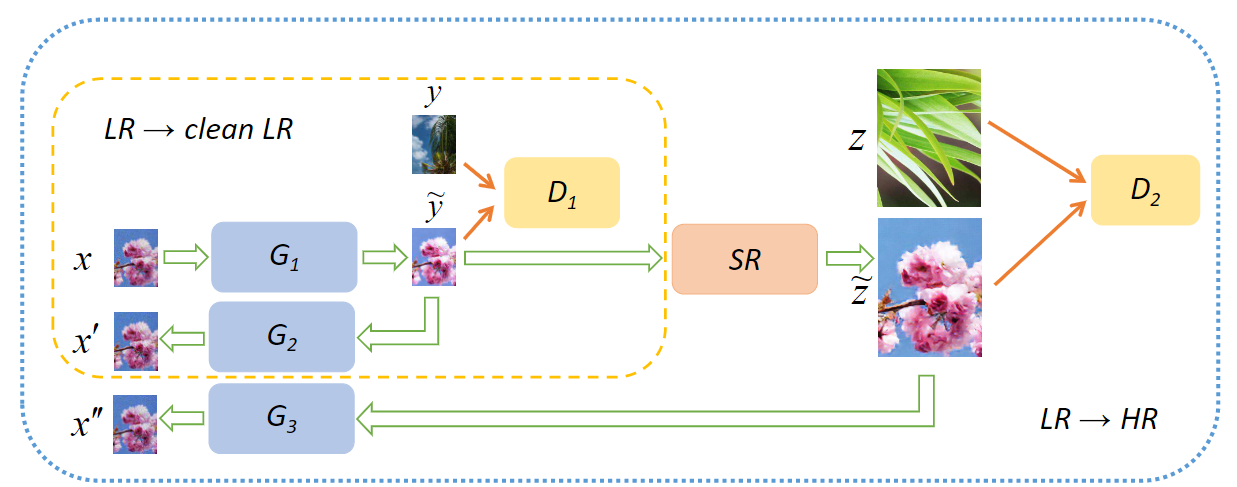
\includegraphics[width=14cm]{./image/GAN.png}
		\caption{研究内容概括}
		\label{fig:label}
	\end{figure}
	
	\subsection{研究步骤}
	\begin{enumerate}
		\item 文献调研。。。;
		\item CUDA编程学习。。。。;
		\item 设计实。。。。;
		\item 优化加速算法。。。。;
		\item 撰写论文,准备答辩;
	\end{enumerate}
	\subsection{创新点挖掘}
	\begin{enumerate}
		\item 。。。。;
		\item 。。。。。。
		\item 。。。。。。
	\end{enumerate}
	
	\section{进度安排}
	
	\subsection{已完成工作}
	\begin{enumerate}
		\item 文献调研\cite{wang2020deep,2021KnowledgeDistillation,lightfieldcamera}。。。。。。
		\item 针。。。。。。
		\item 复现。。。。。
		\item 部分损失函数的改进尝试实验,还未取得较好的效果。
		
	\end{enumerate}
	\subsection{后续工作计划}
	\begin{itemize}
		\item 2021年6月以前:文献调研,学习C++。。。。
		
		\item 2021年07月—2021年12月:。。。。。。
		
		\item 2022年01月—2022年05月:。。。。。
		
		\item 2022年06月—2022年12月:。。。。。。。。。。
	\end{itemize}
	
	\addcontentsline{toc}{section}{参考文献}
	
	\bibliography{reference}
\end{sloppypar}
	
\end{document}